\documentclass[11pt, a4paper]{article}

\usepackage[margin=1in]{geometry}
\usepackage{amsmath, amssymb, amsfonts}
\usepackage{graphicx}
\usepackage{caption}
\usepackage{subcaption}

\usepackage{algorithm}
\usepackage{algpseudocode}
\usepackage{csquotes}
\usepackage{graphicx}
\usepackage{xcolor}
\definecolor{thesisblue}{RGB}{20, 68, 106}
\definecolor{thesisgray}{RGB}{80, 80, 80}
\usepackage{lmodern}
\usepackage{microtype}
\usepackage{amsmath}   
\usepackage{array}
\usepackage{amssymb}   
\usepackage{amsfonts}  
\usepackage{multicol}  
\usepackage{booktabs} 
\usepackage{tabularx}

\usepackage{enumitem}  
\usepackage{lipsum}     
\usepackage{caption}
\usepackage{subcaption}
\usepackage{colortbl}
\usepackage{longtable} 
\usepackage{lscape}   

\usepackage{pgfplots} 
\usepgfplotslibrary{groupplots}
\pgfplotsset{compat=1.18} 
\usepackage{float}

\usepackage{etoolbox}
\usepackage{xcolor} 
\usepackage{tabularray}

\usepackage{tikz}
\usetikzlibrary{
    positioning,
    fit,
    arrows.meta,
    shapes.geometric,
    calc,
    matrix,
    patterns,
    shadows,
    backgrounds,
    decorations.pathreplacing,
    shapes.misc
}

\tikzset{
    cuboid/.style={
        shape=trapezium,
        trapezium left angle=70,
        trapezium right angle=-70,
        shape border rotate=90,
        minimum width=2.2cm,
        minimum height=1cm,
        draw, thick,
        align=center,
        font=\small
    },
    cuboidfill/.style={
        fill=blue!20
    },
    trainable/.style={
        fill=orange!30
    },
    block/.style={
        rectangle, draw, thick,
        minimum width=3cm, minimum height=1.5cm, align=center,
        rounded corners=3pt
    },
    op/.style={
        circle, draw, thick, fill=gray!10, minimum size=0.8cm
    },
    arrow/.style={
        -Stealth, thick, draw=black!80
    },
    loraarrow/.style={
        -Stealth, thick, draw=orange!80!black
    },
    lorabox/.style={
        draw=orange!70!black, dashed, thick,
        inner sep=6pt, rounded corners
    },
    blocktitle/.style={
        font=\sffamily\bfseries\small, text=black!90
    }, 
    outnode/.style={
        rectangle, draw, fill=blue!10, rounded corners, minimum height=1cm
    }
}

\begin{document}

\section*{Diagram Library}

\begin{figure}[htbp]
\centering
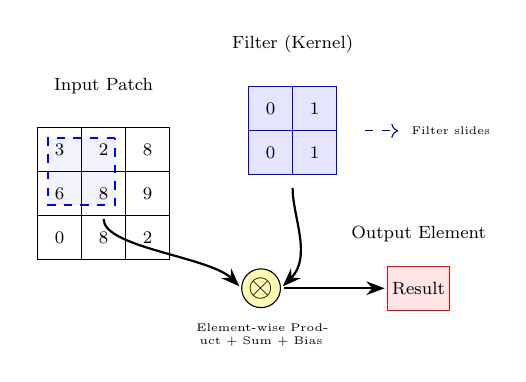
\begin{tikzpicture}[
    scale=0.8, every node/.style={scale=0.8, font=\footnotesize, align=center},
    cell/.style={rectangle, draw, minimum size=0.7cm, inner sep=2pt},
    filter_cell/.style={rectangle, draw=blue, fill=blue!10, minimum size=0.7cm, inner sep=2pt},
    output_cell/.style={rectangle, draw=red, fill=red!10, minimum size=0.7cm, inner sep=2pt},
    op_symbol/.style={circle, draw, fill=yellow!30, minimum size=0.5cm, inner sep=1pt, font=\Large},
    arrow_style/.style={-Stealth, thick, shorten >=1pt, shorten <=1pt}
  ]

    \matrix (input_patch) [matrix of nodes, nodes={cell}, column sep=-\pgflinewidth, row sep=-\pgflinewidth, anchor=center] at (0,0) {
        \pgfmathrandominteger{\val}{0}{9}\val & \pgfmathrandominteger{\val}{0}{9}\val & \pgfmathrandominteger{\val}{0}{9}\val \\
        \pgfmathrandominteger{\val}{0}{9}\val & \pgfmathrandominteger{\val}{0}{9}\val & \pgfmathrandominteger{\val}{0}{9}\val \\
        \pgfmathrandominteger{\val}{0}{9}\val & \pgfmathrandominteger{\val}{0}{9}\val & \pgfmathrandominteger{\val}{0}{9}\val \\
    };
    \node[above=0.2cm of input_patch] {Input Patch};

    \matrix (filter) [matrix of nodes, nodes={filter_cell}, column sep=-\pgflinewidth, row sep=-\pgflinewidth, anchor=center] at (3,1) { % Positioned slightly above center
        \pgfmathrandominteger{\w}{0}{1}\w & \pgfmathrandominteger{\w}{0}{1}\w \\
        \pgfmathrandominteger{\w}{0}{1}\w & \pgfmathrandominteger{\w}{0}{1}\w \\
    };
    \node[above=0.2cm of filter] {Filter (Kernel)};

    \begin{scope}[on background layer]
        \node [fit=(input_patch-1-1) (input_patch-2-2), draw=blue, thick, fill=blue!5, inner sep=-1pt, dashed] {};
    \end{scope}

    \node[op_symbol] (operation) at (2.5, -1.5) {$\otimes$}; % Using \otimes for convolution-like operation
    \node[below=0.1cm of operation, text width=2.5cm, font=\tiny] {Element-wise Product + Sum + Bias};

    \node[output_cell] (output_value) at (5, -1.5) {Result};
    \node[above=0.2cm of output_value] {Output Element};

    \draw[arrow_style] (input_patch-2-2.south) .. controls +(0,-0.5) and +(-0.5,0.5) .. (operation.west);
    \draw[arrow_style] (filter.south) .. controls +(0,-0.5) and +(0.5,0.5) .. (operation.east);
    \draw[arrow_style] (operation.east) -- (output_value.west);

    \draw[->, blue!70!black, dashed, shorten >=2pt, shorten <=2pt] (filter.east) ++(0.2,0) -- ++(0.7,0) node[right, font=\tiny, black] {Filter slides};

\end{tikzpicture}
\caption{Principle of the convolution operation.}
\label{fig:convolution_simplified}
\end{figure}
\vspace{2cm}

\begin{figure}[htbp]
\centering
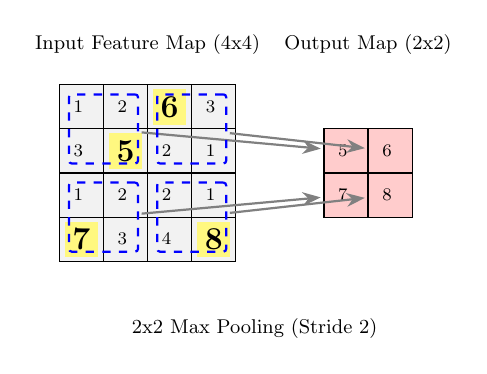
\begin{tikzpicture}[
    scale=0.8, every node/.style={scale=0.8, font=\footnotesize, align=center},
    input_cell/.style={rectangle, draw, minimum size=0.7cm, inner sep=2pt, fill=gray!10},
    max_val_cell_style/.style={fill=yellow!50, font=\bfseries\Large}, % Style for the max value, larger font
    output_cell/.style={rectangle, draw, minimum size=0.7cm, inner sep=2pt, fill=red!20},
    window_highlight/.style={draw=blue, thick, dashed, inner sep=-0.5pt, rounded corners=1pt},
    arrow_style/.style={-Stealth, thick, shorten >=1pt, shorten <=1pt, gray}
  ]

    \node[above=0.2cm, font=\small] (input_label) at (1,2.5) {Input Feature Map (4x4)};
    \matrix (input_map) [matrix of nodes, nodes={input_cell},
                         column sep=-\pgflinewidth, row sep=-\pgflinewidth,
                         anchor=center] at (1,1) {
      1 & 2 & 6 & 3 \\
      3 & 5 & 2 & 1 \\
      1 & 2 & 2 & 1 \\
      7 & 3 & 4 & 8 \\
    };

    \node at (input_map-2-2) [max_val_cell_style] {5};
    \node at (input_map-1-3) [max_val_cell_style] {6};
    \node at (input_map-4-1) [max_val_cell_style] {7};
    \node at (input_map-4-4) [max_val_cell_style] {8};

    \node[above=0.2cm, font=\small] (output_label) at (4.5,2.5) {Output Map (2x2)};
    \matrix (output_map) [matrix of nodes, nodes={output_cell},
                          column sep=-\pgflinewidth, row sep=-\pgflinewidth,
                          anchor=center] at (4.5,1) { 
      5 & 6 \\
      7 & 8 \\
    };

    \node [window_highlight, fit=(input_map-1-1) (input_map-2-2)] (w1) {};
    \draw[arrow_style] (w1) -- (output_map-1-1);

    \node [window_highlight, fit=(input_map-1-3) (input_map-2-4)] (w2) {};
    \draw[arrow_style] (w2) -- (output_map-1-2);

    \node [window_highlight, fit=(input_map-3-1) (input_map-4-2)] (w3) {};
    \draw[arrow_style] (w3) -- (output_map-2-1);

    \node [window_highlight, fit=(input_map-3-3) (input_map-4-4)] (w4) {};
    \draw[arrow_style] (w4) -- (output_map-2-2);

    \node[below=0.5cm of input_map.south, xshift=1.7cm, font=\small] {2x2 Max Pooling (Stride 2)};

\end{tikzpicture}
\caption{Max pooling with 2x2 windows from input to output.}
\label{fig:max_pooling_simple}
\end{figure}
\vspace{2cm}


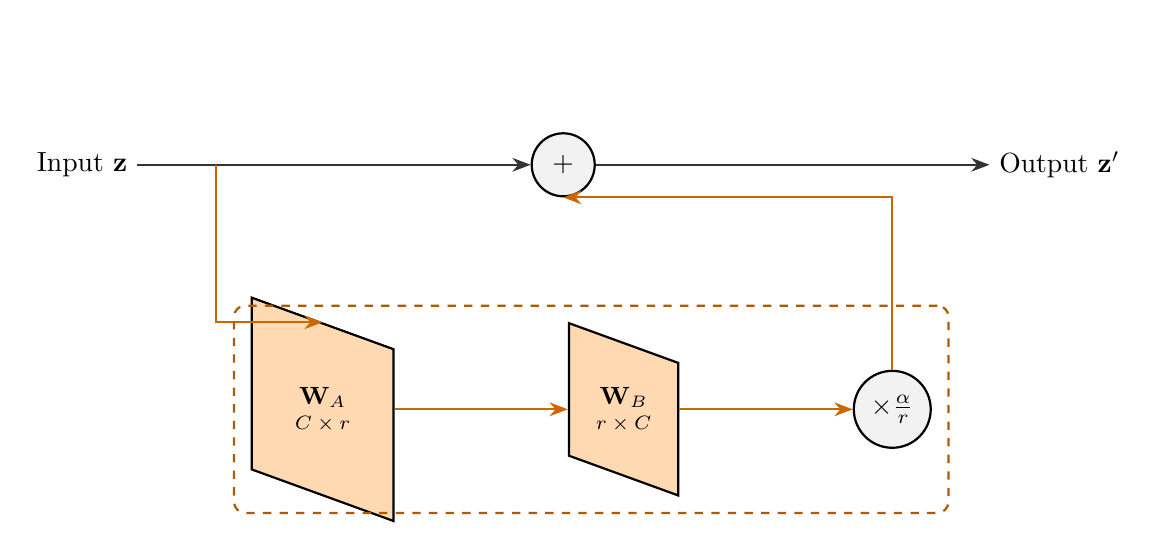
\begin{tikzpicture}[node distance=2cm and 2.2cm]
    \node (input) {Input $\mathbf{z}$};
    \node[op, right=5cm of input] (add) {$+$};
    \node[right=5cm of add] (output) {Output $\mathbf{z}'$};

    \coordinate (lora_center) at ($(input)!0.5!(add)$);
    \node[cuboid, trainable, below=2cm of lora_center, minimum height=1.8cm] (lora_a) 
        {$\mathbf{W}_A$ \\[-2pt] {\scriptsize $C \times r$}};
    \node[cuboid, trainable, right=2.2cm of lora_a, minimum height=1.2cm] (lora_b) 
        {$\mathbf{W}_B$ \\[-2pt] {\scriptsize $r \times C$}};
    \node[op, right=2.2cm of lora_b] (scale) {$\times \tfrac{\alpha}{r}$};

    \draw[arrow] (input.east) -- (add.west);
    \draw[arrow] (add.east) -- (output.west);
    \draw[loraarrow] (input.east) ++(1.0,0) |- (lora_a.north);
    \draw[loraarrow] (lora_a.east) -- (lora_b.west);
    \draw[loraarrow] (lora_b.east) -- (scale.west);
    \draw[loraarrow] (scale.north) |- (add.south);

    \node[lorabox, fit=(lora_a)(lora_b)(scale)] {};
    \node[blocktitle, above=1.5cm of lora_center] {};
\end{tikzpicture}
\vspace{2cm}

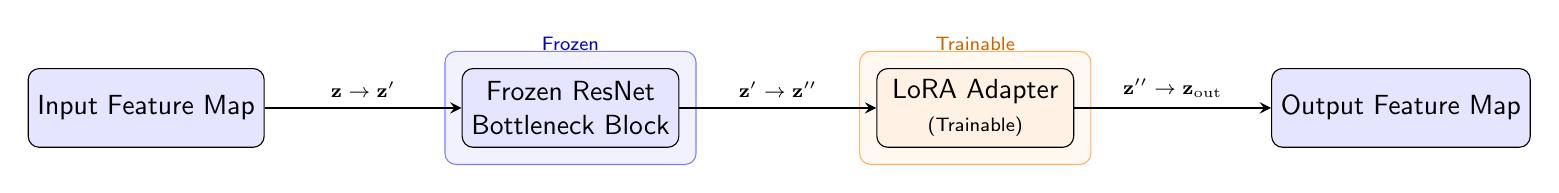
\begin{tikzpicture}[node distance=1.5cm and 2.5cm, 
	block/.style={rectangle, draw, fill=blue!10, rounded corners, minimum height=1cm, minimum width=2.5cm, align=center},
	adapter/.style={rectangle, draw, fill=orange!10, rounded corners, minimum height=1cm, minimum width=2.5cm, align=center},
	arrow/.style={->, thick, >=stealth},
	font=\sffamily
	]
	
	% NODES
	\node (input) [block] {Input Feature Map};
	\node (resnet) [block, right=of input] {Frozen ResNet \\ Bottleneck Block};
	\node (lora) [adapter, right=of resnet] {LoRA Adapter \\ {\scriptsize (Trainable)}};
	\node (output) [block, right=of lora] {Output Feature Map};
	
	% ARROWS
	\draw[arrow] (input) -- (resnet) node[midway, above, font=\scriptsize] {$\mathbf{z} \rightarrow \mathbf{z}'$};
	\draw[arrow] (resnet) -- (lora) node[midway, above, font=\scriptsize] {$\mathbf{z}' \rightarrow \mathbf{z}''$};
	\draw[arrow] (lora) -- (output) node[midway, above, font=\scriptsize] {$\mathbf{z}'' \rightarrow \mathbf{z}_{\text{out}}$};
	
	% BACKGROUND HIGHLIGHT ZONES 
	\begin{scope}[on background layer]
		\node[draw=blue!50, fill=blue!5, rounded corners, inner sep=6pt, fit=(resnet)] {};
		\node[draw=orange!60, fill=orange!5, rounded corners, inner sep=6pt, fit=(lora)] {};
	\end{scope}
	
	% LABELS 
	\node[font=\sffamily\scriptsize, text=blue!80!black, above=0.1cm of resnet.north] {Frozen};
	\node[font=\sffamily\scriptsize, text=orange!80!black, above=0.1cm of lora.north] {Trainable};
	
\end{tikzpicture}

\vspace{2cm}

\begin{tikzpicture}[
	node distance=1.5cm and 0.7cm,
	every node/.style={font=\scriptsize\sffamily},
	dimlabel/.style={below, font=\tiny\ttfamily\bfseries, text=black!80, yshift=-4mm},
	backbone_block/.style={rectangle, draw=blue!50!black, thick, fill=blue!6, rounded corners, minimum width=2.4cm, minimum height=0.95cm, align=center},
	lora_block/.style={rectangle, draw=orange!60!black, thick, fill=orange!22, rounded corners, minimum width=2.8cm, minimum height=1.3cm},
	stem_block/.style={rectangle, draw=purple!40!black, thick, fill=purple!12, rounded corners, minimum width=2.4cm, minimum height=0.95cm, align=center},
	trainable_block/.style={rectangle, draw=purple!90!black, thick, fill=purple!20, rounded corners, minimum width=2.4cm, minimum height=0.95cm, align=center},
	arrow/.style={-Stealth, thick, draw=black!80}
	]
	
	% --- INPUT ---
	\node[draw, thick, minimum width=1.6cm, minimum height=1.6cm] (input) 
	{\includegraphics[width=1.5cm]{DIAGRAMS/input.png}};
	\node[dimlabel] at (input.south) {512x512x3};
	
	% --- STEM ---
	\node[stem_block, right=of input] (stem) {Stem};
	\node[dimlabel] at (stem.south) {128x128x64};
	
	% --- STAGE 1 (LoRA wrapping Stage) ---
	\node[lora_block, right=of stem] (l1) {};
	\node[backbone_block, at=(l1)] (s1) {Stage 1};
	\node[dimlabel] at (l1.south) {128x128x256};
	
	% --- STAGE 2 (LoRA wrapping Stage) ---
	\node[lora_block, right=of l1] (l2) {};
	\node[backbone_block, at=(l2)] (s2) {Stage 2};
	\node[dimlabel] at (l2.south) {64x64x512};
	
	% --- STAGE 3 (LoRA wrapping Stage) ---
	\node[lora_block, right=of l2] (l3) {};
	\node[backbone_block, at=(l3)] (s3) {Stage 3};
	\node[dimlabel] at (l3.south) {32x32x1024};
	
	% --- STAGE 4 (LoRA wrapping Stage) ---
	\node[lora_block, right=of l3] (l4) {};
	\node[trainable_block, at=(l4)] (s4) {Stage 4};
	\node[dimlabel] at (l4.south) {16x16x2048};
	
	% --- GLOBAL FEATURE VECTOR ---
	\node[circle, draw, thick, fill=gray!10, below=1.4cm of l4] (gap) {GAP};
	\node[rectangle, draw, thick, fill=green!10, rounded corners,
	minimum height=1.6cm, minimum width=0.3cm, below=0.8cm of gap] (vector) {};
	\node[below=0.2cm of vector] {\scriptsize 2048-D};
	\node[left=0.6cm of vector] (out_global) {\textbf{Global Vector}};
	
	% --- MULTI-SCALE OUTPUTS ---
	\node[above=1.2cm of l1] (out_c1) {\textbf{C1}};
	\node[above=1.2cm of l2] (out_c2) {\textbf{C2}};
	\node[above=1.2cm of l3] (out_c3) {\textbf{C3}};
	\node[above=1.2cm of l4] (out_c4) {\textbf{C4}};
	\node[above=0.25cm of out_c1] {\tiny 128x128x256};
	\node[above=0.25cm of out_c2] {\tiny 64x64x512};
	\node[above=0.25cm of out_c3] {\tiny 32x32x1024};
	\node[above=0.25cm of out_c4] {\tiny 16x16x2048};
	
	% --- ARROWS (main flow) ---
	\draw[arrow] (input) -- (stem);
	\draw[arrow] (stem) -- (l1);
	\draw[arrow] (l1) -- (l2);
	\draw[arrow] (l2) -- (l3);
	\draw[arrow] (l3) -- (l4);
	\draw[arrow] (l4) -- (gap);
	\draw[arrow] (gap) -- (vector);
	\draw[arrow] (vector.west) -- (out_global.east);
	
	% --- ARROWS (multi-scale outputs) ---
	\draw[arrow] (l1.north) -- (out_c1.south);
	\draw[arrow] (l2.north) -- (out_c2.south);
	\draw[arrow] (l3.north) -- (out_c3.south);
	\draw[arrow] (l4.north) -- (out_c4.south);
	
	% --- BACKGROUND PATH (Blue frozen backbone path) ---
	\begin{scope}[on background layer]
		\node[draw=blue!50, fill=blue!5, rounded corners, inner sep=8pt,
		fit=(stem) (l1) (l2) (l3) (l4)] {};
	\end{scope}
	
\end{tikzpicture}
\vspace{2cm}


    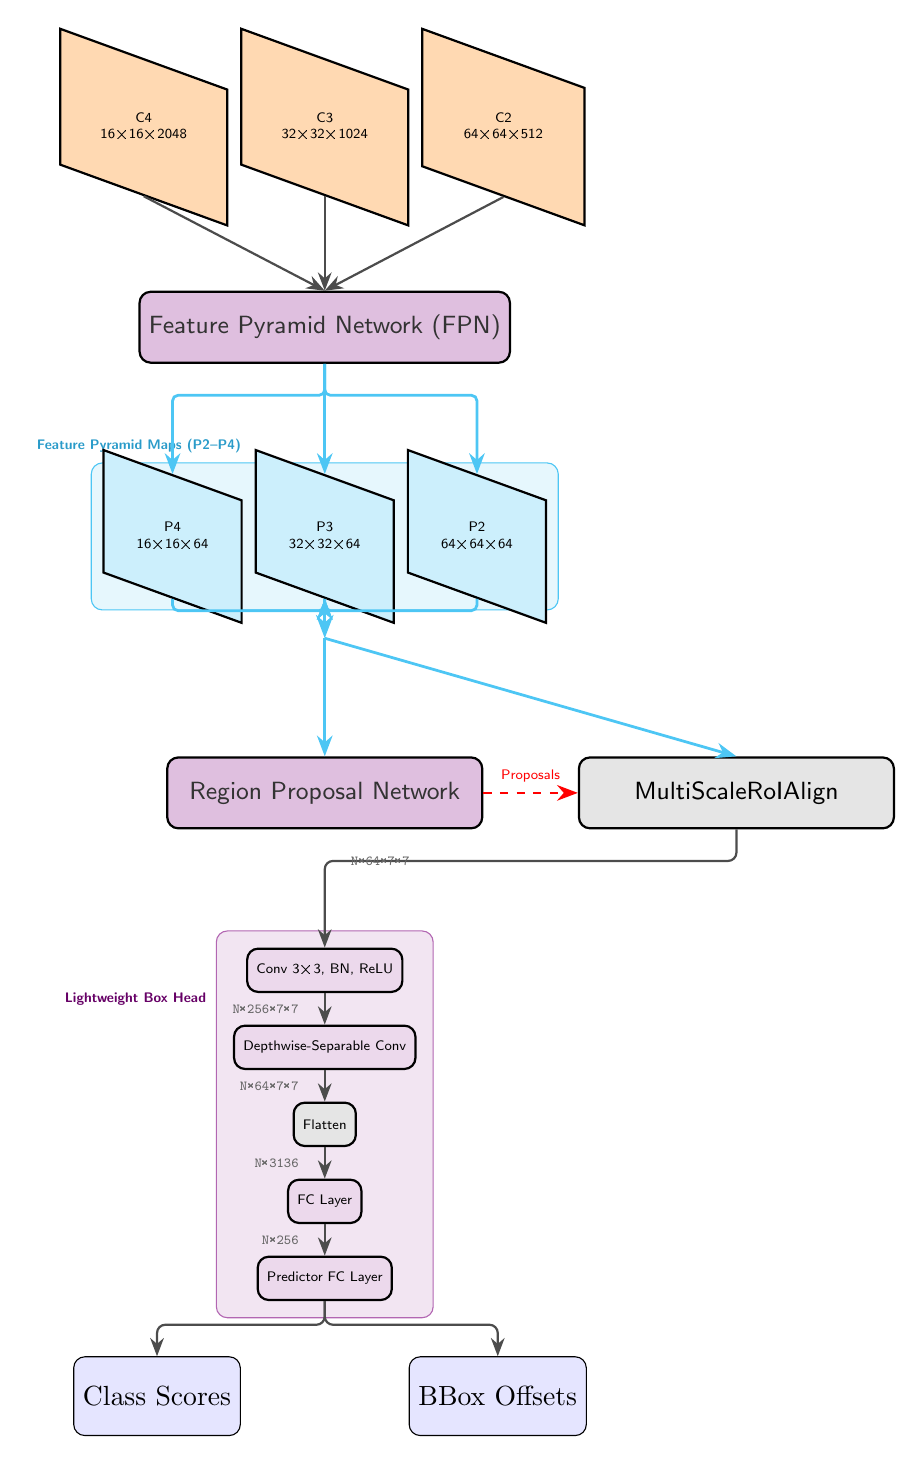
\begin{tikzpicture}[
        node distance=1.2cm and 0.8cm,
        block/.style={rectangle, draw, thick, fill=gray!20, rounded corners, minimum width=4cm, minimum height=0.9cm, align=center, font=\sffamily\small},
        trainable_block/.style={block, fill=violet!25, text=black!80},
        op/.style={rectangle, draw, thick, fill=violet!15, rounded corners, font=\sffamily\tiny, minimum height=0.55cm},
        arrow/.style={-Stealth, thick, draw=black!70, rounded corners=3pt},
        feat_map/.style={cuboid, cuboidfill, minimum width=2.5cm, minimum height=0.55cm, font=\sffamily\tiny, fill=orange!30},
        pyramid_map/.style={cuboid, cuboidfill, minimum width=2.2cm, minimum height=0.5cm, font=\sffamily\tiny, fill=cyan!20},
        out/.style={rectangle, draw, thick, fill=green!25, rounded corners, align=center, font=\sffamily\tiny, minimum width=2.8cm},
        % Custom arrows
        pyramid_arrow/.style={-Stealth, thick, draw=cyan!70, rounded corners=2pt, line width=1pt},
        proposal_arrow/.style={-Stealth, thick, draw=red!70!black, dashed, rounded corners=2pt, line width=1pt, font=\sffamily\tiny, red},
        dim_label_right/.style={midway, right, font=\tiny\ttfamily, text=black!60, xshift=2mm},
        dim_label_left/.style={midway, left, font=\tiny\ttfamily, text=black!60, xshift=-2mm}
    ]
    
    % TITLE
    \node[blocktitle] (title) {};
    
    % INPUTS
    \node[feat_map] (c3) {C3\\32×32×1024};
    \node[feat_map, left=0.15cm of c3] (c4) {C4\\16×16×2048};
    \node[feat_map, right=0.15cm of c3] (c2) {C2\\64×64×512};

    % FPN 
    \node[trainable_block, below=1.2cm of c3] (fpn) {Feature Pyramid Network (FPN)};

    % Pyramid Maps (P2–P4) 
    \node[pyramid_map] (p3) [below=1.4cm of fpn] {P3\\32×32×64};
    \node[pyramid_map, left=0.15cm of p3] (p4) {P4\\16×16×64};
    \node[pyramid_map, right=0.15cm of p3] (p2) {P2\\64×64×64};

    % Pyramid zone
    \begin{scope}[on background layer]
        \node[draw=cyan!70, fill=cyan!10, rounded corners, inner sep=4pt,
              fit=(p2) (p3) (p4),
              label={[font=\sffamily\bfseries\tiny, text=cyan!80!black]135:Feature Pyramid Maps (P2–P4)}] {};
    \end{scope}
    
    % RPN & RoIAlign
    \node[trainable_block, below=2cm of p3] (rpn) {Region Proposal Network};
    \node[block, right=1.2cm of rpn] (roi_align) {MultiScaleRoIAlign};

    % Lightweight Box Head
    \node[op, below=1.5cm of rpn, fill=violet!15] (head_conv) {Conv 3×3, BN, ReLU};
    \node[op, below=0.4cm of head_conv] (head_ds_conv) {Depthwise-Separable Conv};
    \node[op, below=0.4cm of head_ds_conv, fill=gray!20] (head_flatten) {Flatten};
    \node[op, below=0.4cm of head_flatten] (head_fc) {FC Layer};
    \node[op, below=0.4cm of head_fc] (predictor) {Predictor FC Layer};
    
    % Outputs
    \node[outnode, below left=0.7cm and 0.2cm of predictor] (class_out) {Class Scores};
    \node[outnode, below right=0.7cm and 0.2cm of predictor] (bbox_out) {BBox Offsets};

    % Connections
    % Backbone -> FPN
    \draw[arrow] (c2.south) -- (fpn.north);
    \draw[arrow] (c3.south) -- (fpn.north);
    \draw[arrow] (c4.south) -- (fpn.north);
    
    % FPN -> Pyramid Maps
    \draw[pyramid_arrow] (fpn.south) -- ++(0,-0.4) -| (p2.north);
    \draw[pyramid_arrow] (fpn.south) -- (p3.north);
    \draw[pyramid_arrow] (fpn.south) -- ++(0,-0.4) -| (p4.north);

    % Pyramid -> bus -> RPN & RoIAlign
    \coordinate (bus_top) at ($(p4.south)!0.5!(p2.south)$);
    \coordinate (bus_bottom) at ($(bus_top)+(0,-0.5cm)$);
    \draw[pyramid_arrow, line width=1.2pt] (bus_top) -- (bus_bottom);
    \draw[pyramid_arrow] (p2.south) -- ++(0,-0.15) -| (bus_top);
    \draw[pyramid_arrow] (p3.south) -- ++(0,-0.15) -| (bus_top);
    \draw[pyramid_arrow] (p4.south) -- ++(0,-0.15) -| (bus_top);
    \draw[pyramid_arrow] (bus_bottom) -- (rpn.north);
    \draw[pyramid_arrow] (bus_bottom) -- (roi_align.north);

    % RPN -> RoIAlign (Proposals)
    \draw[proposal_arrow] (rpn.east) -- node[midway, above, font=\sffamily\tiny] {Proposals} (roi_align.west);
    
    % RoIAlign -> Box Head 
    \draw[arrow] (roi_align.south) -- ++(0,-0.4) -| node[dim_label_right] {N×64×7×7} (head_conv.north);
    \draw[arrow] (head_conv) -- node[dim_label_left] {N×256×7×7} (head_ds_conv);
    \draw[arrow] (head_ds_conv) -- node[dim_label_left] {N×64×7×7} (head_flatten);
    \draw[arrow] (head_flatten) -- node[dim_label_left] {N×3136} (head_fc);
    \draw[arrow] (head_fc) -- node[dim_label_left] {N×256} (predictor);

    % Final Outputs
    \draw[arrow] (predictor.south) -- ++(0,-0.3) -| (class_out.north);
    \draw[arrow] (predictor.south) -- ++(0,-0.3) -| (bbox_out.north);

    \begin{scope}[on background layer]
        \node[draw=violet!60, fill=violet!10, rounded corners, inner sep=6pt,
              fit=(head_conv) (head_ds_conv) (head_flatten) (head_fc) (predictor),
              label={[font=\sffamily\bfseries\tiny, text=violet!80!black]135:Lightweight Box Head}] {};
    \end{scope}

\end{tikzpicture}

\vspace{2cm}

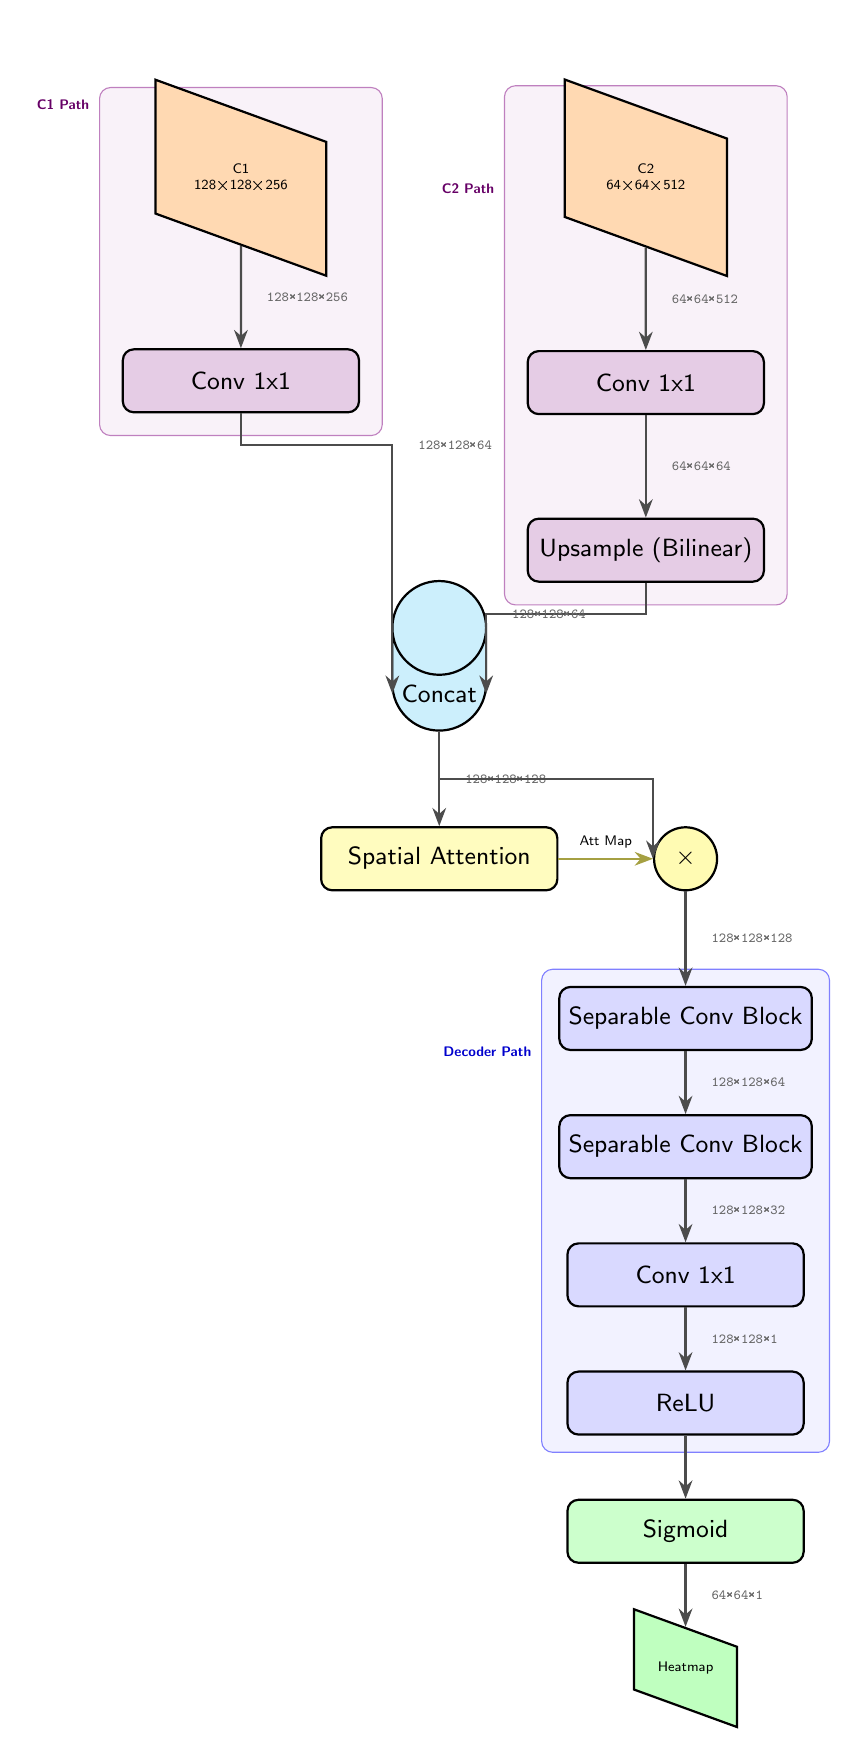
\begin{tikzpicture}[
    node distance=1.3cm and 1.5cm,
    block/.style={rectangle, draw, thick, fill=violet!20, rounded corners, minimum width=3cm, minimum height=0.8cm, align=center, font=\sffamily\small},
    feat_map/.style={cuboid, cuboidfill, minimum width=2.5cm, minimum height=0.55cm, font=\sffamily\tiny, fill=orange!30},
    op/.style={circle, draw, thick, fill=gray!10, minimum size=0.8cm, font=\sffamily\small},
    out_map/.style={cuboid, fill=green!25, minimum width=1.5cm, minimum height=0.4cm, font=\sffamily\tiny},
    arrow/.style={-Stealth, thick, draw=black!70}, % Sharp lines
    dim_label_right/.style={midway, right, font=\tiny\ttfamily, text=black!60, xshift=2mm}
]
    
    % --- TITLE ---
    \node[blocktitle] (title) {};
    
    % --- INPUTS ---
    \node[feat_map, below=0.8cm of title] (c1) {C1\\128×128×256};
    \node[feat_map, right=3cm of c1] (c2) {C2\\64×64×512};

    % --- PROJECTION & FUSION PATH ---
    \node[block, below=of c1] (proj1) {Conv 1x1};
    \node[block, below=of c2] (proj2) {Conv 1x1};
    \node[block, below=of proj2] (upsample) {Upsample (Bilinear)};
    
    \node[op, shape=cylinder, shape border rotate=90, minimum height=0.9cm, fill=cyan!20, below left=0.8cm and 0.5cm of upsample] (concat) {Concat};

    % --- ATTENTION PATH ---
    \node[block, below=1.2cm of concat, fill=yellow!25] (attention) {Spatial Attention};
    \node[op, right=1.2cm of attention, fill=yellow!30] (multiply) {$\times$};

    % --- DECODER PATH (with uniform spacing) ---
    \newcommand{\decoderVspace}{0.8cm} 
    
    \node[block, below=1.2cm of multiply, fill=blue!15] (sep_conv1) {Separable Conv Block};
    \node[block, below=\decoderVspace of sep_conv1, fill=blue!15] (sep_conv2) {Separable Conv Block};
    \node[block, below=\decoderVspace of sep_conv2, fill=blue!15] (final_conv) {Conv 1x1};
    \node[block, below=\decoderVspace of final_conv, fill=blue!15] (relu) {ReLU};
    \node[block, below=\decoderVspace of relu, fill=green!20] (sigmoid) {Sigmoid};

    % --- OUTPUT ---
    \node[out_map, below=\decoderVspace of sigmoid] (output) {Heatmap};
    
    % --- ARROWS & DIMENSIONS ---
    \draw[arrow] (c1) -- node[dim_label_right] {128×128×256} (proj1);
    \draw[arrow] (c2) -- node[dim_label_right] {64×64×512} (proj2);
    
    \draw[arrow] (proj1.south) -- ++(0,-0.4) -| node[dim_label_right] {128×128×64} (concat.west);
    \draw[arrow] (proj2.south) -- node[dim_label_right] {64×64×64} (upsample);
    \draw[arrow] (upsample.south) -- ++(0,-0.4) -| node[dim_label_right] {128×128×64} (concat.east);
    
    \draw[arrow] (concat.south) -- node[dim_label_right] {128×128×128} (attention.north);
    \draw[arrow] (concat.south) -- ++(0,-0.6) -| (multiply.west);
    \draw[arrow, draw=yellow!60!black] (attention.east) -- node[midway, above, font=\sffamily\tiny] {Att Map} (multiply);
    
    \draw[arrow] (multiply.south) -- node[dim_label_right] {128×128×128} (sep_conv1.north);
    \draw[arrow] (sep_conv1.south) -- node[dim_label_right] {128×128×64} (sep_conv2.north);
    \draw[arrow] (sep_conv2.south) -- node[dim_label_right] {128×128×32} (final_conv.north);
    \draw[arrow] (final_conv.south) -- node[dim_label_right] {128×128×1} (relu.north);
    \draw[arrow] (relu.south) -- (sigmoid.north);
    \draw[arrow] (sigmoid.south) -- node[dim_label_right] {64×64×1} (output.north);
    
    % --- ZONES & GROUPING ---
    \begin{scope}[on background layer]
        % Group for Decoder Path
        \node[draw=blue!50, fill=blue!5, rounded corners, inner sep=6pt,
              fit=(sep_conv1) (sep_conv2) (final_conv) (relu),
              label={[font=\sffamily\bfseries\tiny, text=blue!80!black]135:Decoder Path}] {};

        % Group for C1 Path
        \node[draw=violet!50, fill=violet!5, rounded corners, inner sep=8pt,
              fit=(c1) (proj1),
              label={[font=\sffamily\bfseries\tiny, text=violet!80!black]135:C1 Path}] {};
        
        % Group for C2 Path
        \node[draw=violet!50, fill=violet!5, rounded corners, inner sep=8pt,
              fit=(c2) (proj2) (upsample),
              label={[font=\sffamily\bfseries\tiny, text=violet!80!black]135:C2 Path}] {};
    \end{scope}
    
\end{tikzpicture}
\vspace{2cm}

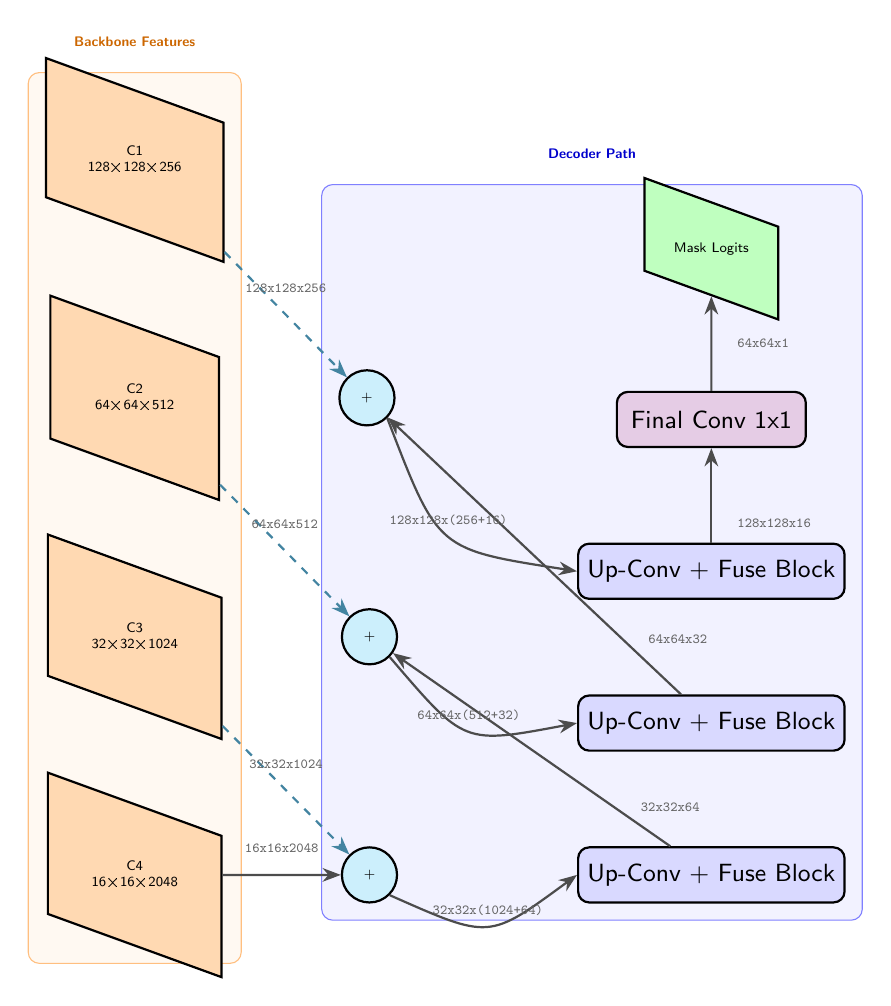
\begin{tikzpicture}[
    node distance=1.2cm and 1cm,
    block/.style={rectangle, draw, thick, fill=blue!15, rounded corners, minimum width=2.4cm, minimum height=0.7cm, align=center, font=\sffamily\small},
    feat_map/.style={cuboid, cuboidfill, minimum width=2.6cm, minimum height=0.55cm, font=\sffamily\tiny, fill=orange!30},
    op/.style={circle, draw, thick, fill=cyan!20, minimum size=0.7cm, font=\sffamily\tiny},
    out_map/.style={cuboid, fill=green!25, minimum width=1.8cm, minimum height=0.45cm, font=\sffamily\tiny},
    arrow/.style={-Stealth, thick, draw=black!70},
    skip_arrow/.style={-Stealth, thick, draw=cyan!60!black, dashed},
    dim_label_above/.style={midway, above, font=\tiny\ttfamily, text=black!60, yshift=1.5mm},
    % ADJUSTMENT: Changed 'midway' to 'pos=0.8' to move labels closer to the end of the arrow
    dim_label_right/.style={pos=0.2, right, font=\tiny\ttfamily, text=black!60, xshift=2mm},
    dim_label_on_arrow/.style={pos=0.5, above, font=\tiny\ttfamily, text=black!60}
]
    
    % --- TITLE ---
    \node[blocktitle, yshift=-0.5cm] (title) {};

    % --- INPUTS (Encoder Path) ---
    \node[feat_map, below=1.2cm of title] (c4_in) {C4\\16×16×2048};
    \node[feat_map, above=of c4_in] (c3_in) {C3\\32×32×1024};
    \node[feat_map, above=of c3_in] (c2_in) {C2\\64×64×512};
    \node[feat_map, above=of c2_in] (c1_in) {C1\\128×128×256};

    % --- DECODER PATH ---
    \node[block, right=4.5cm of c4_in] (d4) {Up-Conv + Fuse Block}; 
    \node[op, right=1.5cm of c4_in] (concat4) {+};

    \node[block, above=of d4] (d3) {Up-Conv + Fuse Block};
    \node[op, right=1.5cm of c3_in] (concat3) {+};

    \node[block, above=of d3] (d2) {Up-Conv + Fuse Block};
    \node[op, right=1.5cm of c2_in] (concat2) {+};
    
    \node[block, above=of d2, fill=violet!20] (final_conv) {Final Conv 1x1};
    \node[out_map, above=of final_conv] (output) {Mask Logits};

    % --- ARROWS (curved + straight) ---
    \draw[arrow] (c4_in) -- node[dim_label_above] {16x16x2048} (concat4);
    \draw[skip_arrow] (c3_in) -- node[dim_label_above] {32x32x1024} (concat4);
    \draw[arrow, bend right=30, looseness=1.5] (concat4.south east) to node[dim_label_on_arrow] {32x32x(1024+64)} (d4.west);

    % The labels on these two arrows will now be closer to the concat nodes
    \draw[arrow] (d4) -- node[dim_label_right] {32x32x64} (concat3);
    \draw[skip_arrow] (c2_in) -- node[dim_label_above] {64x64x512} (concat3);
    \draw[arrow, bend right=30, looseness=1.5] (concat3.south east) to node[dim_label_on_arrow] {64x64x(512+32)} (d3.west);

    \draw[arrow] (d3) -- node[dim_label_right] {64x64x32} (concat2);
    \draw[skip_arrow] (c1_in) -- node[dim_label_above] {128x128x256} (concat2);
    \draw[arrow, bend right=30, looseness=1.5] (concat2.south east) to node[dim_label_on_arrow] {128x128x(256+16)} (d2.west);

    \draw[arrow] (d2) -- node[dim_label_right] {128x128x16} (final_conv);
    \draw[arrow] (final_conv) -- node[dim_label_right, pos=0.5] {64x64x1} (output); % Kept this one centered

    % --- BACKGROUND GROUPING (with zone labels) ---
    \begin{scope}[on background layer]
        \node[draw=orange!50, fill=orange!5, rounded corners, inner sep=6pt,
              fit=(c1_in) (c4_in),
              label={[font=\sffamily\bfseries\tiny, text=orange!80!black, yshift=0.2cm]90:Backbone Features}] {};
        \node[draw=blue!50, fill=blue!5, rounded corners, inner sep=6pt,
              fit=(d2) (d3) (d4) (final_conv) (output) (concat2) (concat3) (concat4),
              label={[font=\sffamily\bfseries\tiny, text=blue!80!black, yshift=0.2cm]90:Decoder Path}] {};
    \end{scope}

\end{tikzpicture}
\vspace{2cm}

\begin{minipage}{0.48\textwidth}
    \centering
    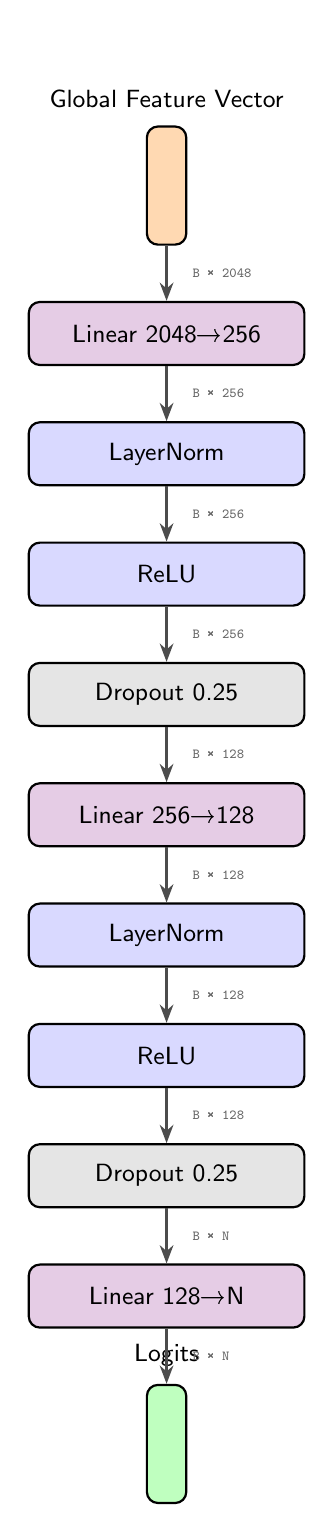
\begin{tikzpicture}[
        node distance=0.7cm,
        block/.style={rectangle, draw, thick, fill=violet!20, rounded corners, minimum width=3.5cm, minimum height=0.8cm, align=center, font=\sffamily\small},
        feat_vec/.style={rectangle, draw, thick, fill=orange!30, rounded corners, minimum height=1.5cm, minimum width=0.5cm},
        out_vec/.style={feat_vec, fill=green!25},
        arrow/.style={-Stealth, thick, draw=black!70},
        dim_label_right/.style={midway, right, font=\tiny\ttfamily\bfseries, text=black!60, xshift=2mm}
    ]

        % Title
        \node[blocktitle] (title) {};

        % Input
        \node[feat_vec, below=1cm of title] (input_vec) {};
        \node[above=0.1cm of input_vec, font=\sffamily\small] {Global Feature Vector};

        % MLP Layers
        \node[block, below=of input_vec] (fc1) {Linear 2048→256};
        \node[block, below=of fc1, fill=blue!15] (norm1) {LayerNorm};
        \node[block, below=of norm1, fill=blue!15] (relu1) {ReLU};
        \node[block, below=of relu1, fill=gray!20] (dropout1) {Dropout 0.25};
        \node[block, below=of dropout1] (fc2) {Linear 256→128};
        \node[block, below=of fc2, fill=blue!15] (norm2) {LayerNorm};
        \node[block, below=of norm2, fill=blue!15] (relu2) {ReLU};
        \node[block, below=of relu2, fill=gray!20] (dropout2) {Dropout 0.25};
        \node[block, below=of dropout2] (fc3) {Linear 128→N};

        % Output
        \node[out_vec, below=of fc3] (output_vec) {};
        \node[above=0.1cm of output_vec, font=\sffamily\small] {Logits};

        % Arrows with full dimensions
        \draw[arrow] (input_vec) -- node[dim_label_right] {B × 2048} (fc1);
        \draw[arrow] (fc1) -- node[dim_label_right] {B × 256} (norm1);
        \draw[arrow] (norm1) -- node[dim_label_right] {B × 256} (relu1);
        \draw[arrow] (relu1) -- node[dim_label_right] {B × 256} (dropout1);
        \draw[arrow] (dropout1) -- node[dim_label_right] {B × 128} (fc2);
        \draw[arrow] (fc2) -- node[dim_label_right] {B × 128} (norm2);
        \draw[arrow] (norm2) -- node[dim_label_right] {B × 128} (relu2);
        \draw[arrow] (relu2) -- node[dim_label_right] {B × 128} (dropout2);
        \draw[arrow] (dropout2) -- node[dim_label_right] {B × N} (fc3);
        \draw[arrow] (fc3) -- node[dim_label_right] {B × N} (output_vec);

    \end{tikzpicture}
\end{minipage}%
\hfill
% --- RIGHT: RoI Classification Head ---
\begin{minipage}{0.48\textwidth}
    \centering
    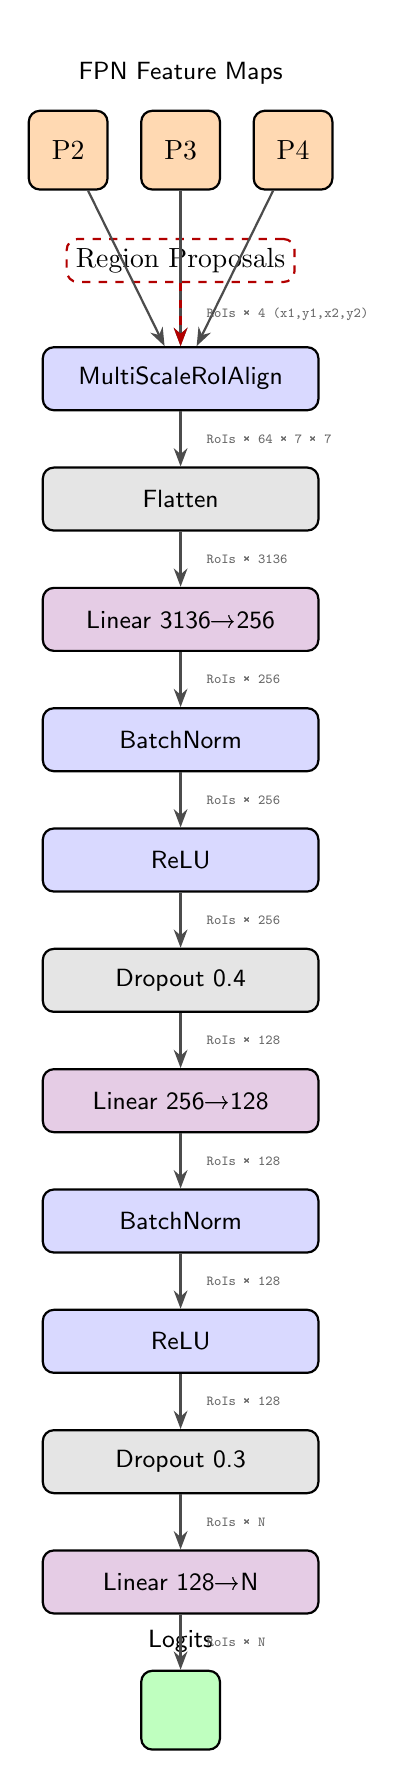
\begin{tikzpicture}[
        node distance=0.7cm,
        block/.style={rectangle, draw, thick, fill=violet!20, rounded corners, minimum width=3.5cm, minimum height=0.8cm, align=center, font=\sffamily\small},
        feat_vec/.style={rectangle, draw, thick, fill=orange!30, rounded corners, minimum height=1cm, minimum width=1cm},
        out_vec/.style={feat_vec, fill=green!25},
        arrow/.style={-Stealth, thick, draw=black!70},
        proposal_arrow/.style={-Stealth, thick, draw=red!70!black, dashed, font=\sffamily\tiny},
        dim_label_right/.style={midway, right, font=\tiny\ttfamily\bfseries, text=black!60, xshift=2mm}
    ]

        % Title
        \node[blocktitle] (title) {};

        % Inputs
        \node[feat_vec, below=0.8cm of title] (p2) {P2};
        \node[feat_vec, right=0.4cm of p2] (p3) {P3};
        \node[feat_vec, right=0.4cm of p3] (p4) {P4};
        \node[above=0.2cm of p3, font=\sffamily\small] {FPN Feature Maps};

        % Proposals
        \node[rectangle, draw, thick, dashed, draw=red!70!black, rounded corners, below=0.6cm of p3] (proposals) {Region Proposals};

        % RoI Pooling
        \node[block, fill=blue!15, below=0.8cm of proposals] (roi_align) {MultiScaleRoIAlign};
        \node[block, fill=gray!20, below=of roi_align] (flatten) {Flatten};

        % MLP
        \node[block, below=of flatten] (mlp1) {Linear 3136→256};
        \node[block, below=of mlp1, fill=blue!15] (norm1) {BatchNorm};
        \node[block, below=of norm1, fill=blue!15] (relu1) {ReLU};
        \node[block, below=of relu1, fill=gray!20] (dropout1) {Dropout 0.4};
        \node[block, below=of dropout1] (mlp2) {Linear 256→128};
        \node[block, below=of mlp2, fill=blue!15] (norm2) {BatchNorm};
        \node[block, below=of norm2, fill=blue!15] (relu2) {ReLU};
        \node[block, below=of relu2, fill=gray!20] (dropout2) {Dropout 0.3};
        \node[block, below=of dropout2] (mlp3) {Linear 128→N};

        % Output
        \node[out_vec, below=of mlp3] (output_vec) {};
        \node[above=0.1cm of output_vec, font=\sffamily\small] {Logits};

        % Arrows with full dimensions
        \draw[arrow] (p2) -- node[dim_label_right] {} (roi_align);
        \draw[arrow] (p3) -- node[dim_label_right] {} (roi_align);
        \draw[arrow] (p4) -- node[dim_label_right] {} (roi_align);
        \draw[proposal_arrow] (proposals) -- node[dim_label_right] {RoIs × 4 (x1,y1,x2,y2)} (roi_align);
        \draw[arrow] (roi_align) -- node[dim_label_right] {RoIs × 64 × 7 × 7} (flatten);
        \draw[arrow] (flatten) -- node[dim_label_right] {RoIs × 3136} (mlp1);
        \draw[arrow] (mlp1) -- node[dim_label_right] {RoIs × 256} (norm1);
        \draw[arrow] (norm1) -- node[dim_label_right] {RoIs × 256} (relu1);
        \draw[arrow] (relu1) -- node[dim_label_right] {RoIs × 256} (dropout1);
        \draw[arrow] (dropout1) -- node[dim_label_right] {RoIs × 128} (mlp2);
        \draw[arrow] (mlp2) -- node[dim_label_right] {RoIs × 128} (norm2);
        \draw[arrow] (norm2) -- node[dim_label_right] {RoIs × 128} (relu2);
        \draw[arrow] (relu2) -- node[dim_label_right] {RoIs × 128} (dropout2);
        \draw[arrow] (dropout2) -- node[dim_label_right] {RoIs × N} (mlp3);
        \draw[arrow] (mlp3) -- node[dim_label_right] {RoIs × N} (output_vec);

    \end{tikzpicture}
\end{minipage}


\end{document}